% !TEX encoding = UTF-8 Unicode
%!TEX root = thesis.tex

\newpage
\section{Background}

Prior to addressing the actual approach and implementation some concepts and terms have to be introduced. Firstly, the term \textit{security concept}, as it is used throughout the thesis, is being described. A definition of \textit{granularity levels} and system abstraction follows. Lastly, a section covers \textit{model transformations} and \textit{aggregation rules} on security attributes.

\subsection{Security}
Many different definitions of security exist. Here, a slightly adapted definition of a \textit{information security management system} (ISMS), as it is found in the ISO/IEC 27001 \cite{iso27001}, is being used.
\begin{quote}
\textit{\glqq The information security management system preserves the confidentiality, integrity and availability
of information by applying a risk management process and gives confidence to interested parties that
risks are adequately managed\grqq}    
\end{quote}

It is also added that the ISMS is integrated into the overall management structure and is vital for many of the organizational processes \cite{iso27001}.

The definition above only covers information security, which in the scope of this thesis, is insufficient. Here, we define security as the preservation of confidentiality, integrity and availability of assets, where assets can be either physical or logical.

\subsection{Enterprise Security}
To define the term \textit{security concept} one has to look at the architecture of enterprises to understand the interconnectivity and interdependence between services, security being one of them. 

\subsubsection{Enterprise Architecture}

Information systems tend to be a very complex artifacts that combine different views and requirements from various stakeholders of different backgrounds \cite{alex}. 

Software, IT platforms and IT related goals in general are covered in an \textit{Information System Architecture} (ISA). ISA does not take any business-driven influences into account and is therefore insufficient when describing the complex dependencies in corporations, especially when it comes to security as described in Subsection \ref{subsec:secarch}.   

\textit{Enterprise Architecture Modeling} tries to overcome such possible difficulties and combines IT related concerns with business and organizational goals and shows possible interrelationships. It therefore provides an approach for an improved understanding of complex enterprise processes \cite{earch}. The Federal Deposit Insurance Corporation (FDIC) published the results of an audit of its own implementation of E-Government principles \cite{fdicaudit} and their division of information technology in Figure \ref{fig:fdic} depicts the interrelations very well. 

\begin{figure}[H]
\centering
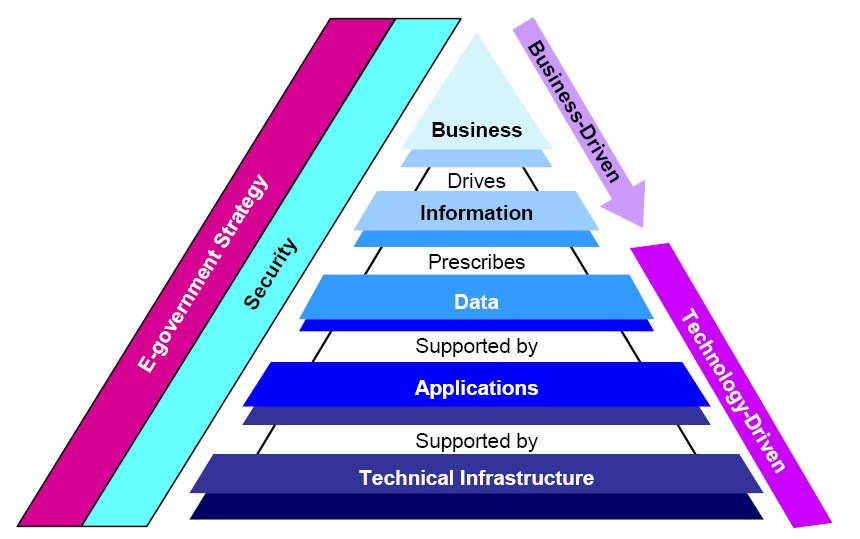
\includegraphics[width=0.75\textwidth]{pictures/fdic.jpg}
\caption{Division of Information Technology by FDIC}
\label{fig:fdic}
\end{figure}

\subsubsection{Security Architecture}
\label{subsec:secarch}

Information Security has often been merely an afterthought in corporations \cite{ansfederal} until a concept of a \textit{Security Architecture}, published in a whitepaper by The Gartner Group \cite{kreizman}, was introduced. According to \cite{kreizman} an \textit{Enterprise Information Security Architecture} (EISA) is an essential tool for improving security processes in corporations. EISA principles stand in a direct relationship with the EA principles and should be validated against them \cite{kreizman}. To highlight this relationship security considerations during phases of the \textit{The Open Group Architecture Framework Architecture Development Method} (TOGAF ADM), which is shown in Figure \ref{fig:togaf}, will be briefly described.

\begin{figure}[H]
\centering
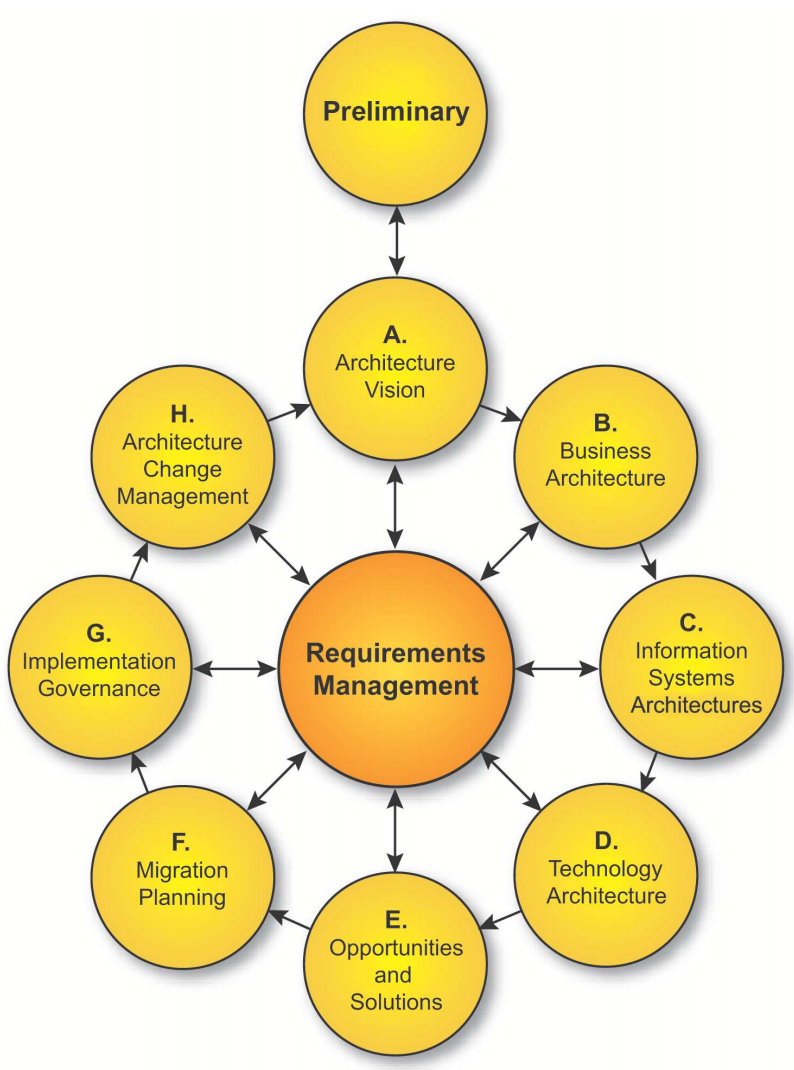
\includegraphics[width=0.6\textwidth]{pictures/togaf_overview.png}
\caption{Overview of the phases of TOGAF}
\label{fig:togaf}
\end{figure}

Security concerns can be found throughout the TOGAF phases which hints at the overall importance of security in corporations. TOGAF combines four architecture domains, the \textit{Business Architecture}, the \textit{Data Architecture}, the \textit{Application Architecture} and the \textit{Technology Architecture}. The following section will depict security considerations of two domains to show possible interrelations.

During the \textit{Business Architecture} phase in the ADM actors and handlers of the system have to be identified. Costs and potential incoveniences because of security measures have to be assessed as well. In general one can say that the impacts of security/insecurity on the business/product are being highlighted. It is tried to put an emphasis on security as early as possible to prevent costly changes in later phases in the ADM.

During the \textit{Information System Architecture} phase the classification levels of processed data have to be determined and documented. Direct dependencies to the \textit{Business Architecture} are also listed, e.g. the identification of information lifespan according to business goals and regulations. 

Similar relations can be found for security considerations from various phases of the ADM. This once again shows the overall presence of security and the high level of complexity within an enterprise.

\subsubsection{Common Criteria}
The overview of TOGAF showed the importance of security in corporations. The following section will present a way of modeling security concerns for an asset of interest.

Common Criteria proposes an evaluation by using a so called \textit{Security Target} (ST), a construct that encapsulates the \textit{Target of Evaluation} (TOE), threats to the TOE and countermeasures \cite{commoncriteria}. The goal of the evaluation is to show that the used countermeasures are sufficient to counter potential threats and thus implying that the TOE is sufficiently protected.

\begin{figure}[H]
\centering
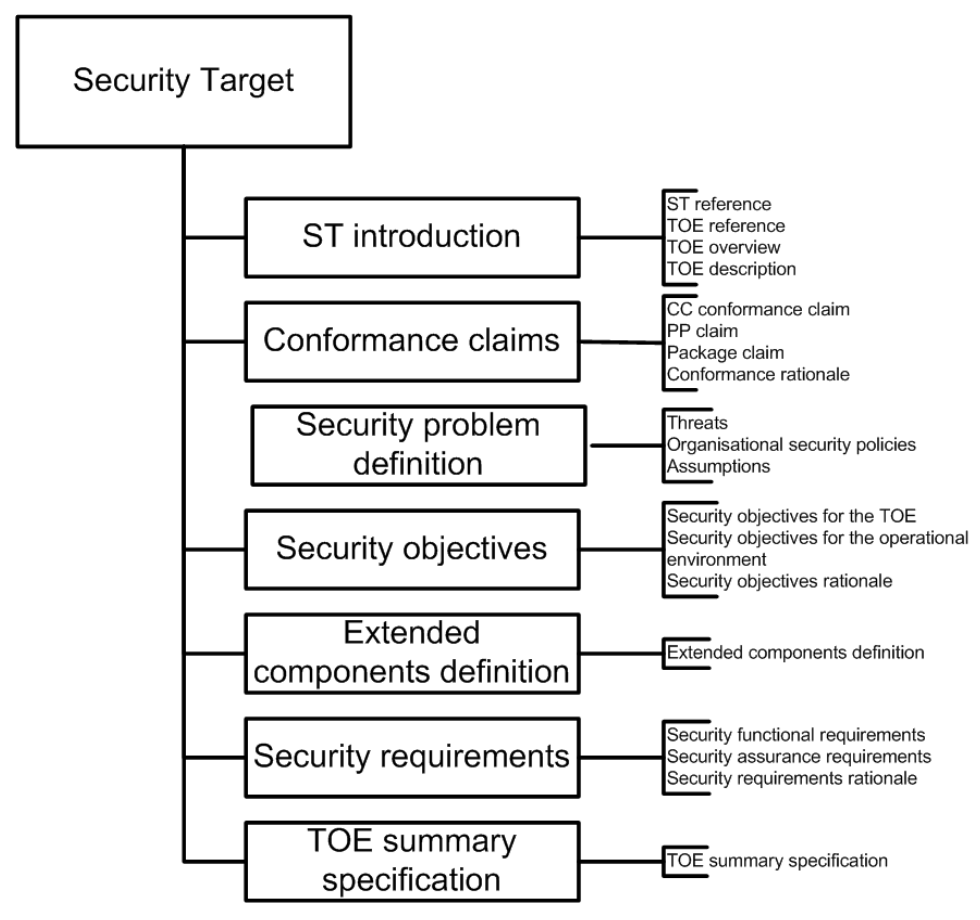
\includegraphics[width=0.85\textwidth]{pictures/sectarget.png}
\caption{Overview of the Security Target contents}
\label{fig:sectarget}
\end{figure}

A description of all the contents of a ST is unnecessary here and only the key security attributes of a ST that will be used to construct a \textit{Security Concept} (Subsection \ref{subsubsec:secconc}) are being introduced.

The \textit{Security Problem Definition} defines, as the name suggests, the security problem that is being addressed. Apart from containing guidelines and assumptions it contains \textit{Threats} which are \textit{\glqq[...] adverse actions performed by a threat agent on an asset\grqq} (\cite{iso27001}, p. 66).

A \textit{Security Objective} is an abstract solution to the previously defined security problem. There exists a possibility to divide the \textit{Security Objectives} into part wise solutions, one being the \textit{Security Objectives for the TOE} and the other being the \textit{Security Objectives for the Operational Environment}. Moreover does the ST contain traces showing which objectives address which threats, guidelines and assumptions and a set showing that all threats, guidelines and assumptions are addressed by the security objective.

\textit{Security Functional Requirements} (SFR) are a more detailed translation of the previously defined \textit{Security Objective}. Despite being more detailed, SFR have to be still independent from specific technical solutions. 

Lastly, STs contain a TOE summary specification where it is stated how the TOE meets all the SFRs and how exactly those requirements are met on a technical level.

\subsubsection{Security Concept}
\label{subsubsec:secconc}

The term \textit{Security Concept}, as it is defined here, is based on the constructs introduced in the previous chapters, namely \textit{Security Architecture} and \textit{Security Target}. An overview follows. 

\textit{Assets} are the to be secured objects of interest, i.e. TOE according to Common Criteria. \textit{Assets} can be either logical or physical and can be grouped to sets, if needed.

\textit{Security Goals} (SG) is the equivalent to the \textit{Security Objective}. A valid SG must address an \textit{Asset} and a \textit{Security Goal Class} that defines the actual purpose of the SG. In general the set of \textit{Security Goal Classes} consists of \textit{Confidentiality}, \textit{Integrity} and \textit{Availability} but can also be expanded by further classes such as \textit{Authenticity}.

\textit{Threats} serve the same purpose as proposed by the Common Criteria. They are adverse actions performed by an entity against an \textit{Asset}. 

This information is all brought together in \textit{Security Requirements} that are defined in natural language and show the interrelationships between elements. A \textit{Security Goal} has to be mentioned as well as an \textit{Asset} and a \textit{Threat} against which the object of interest should be protected. Lastly, \textit{Controls} are the technical measures that counter or minimize the \textit{Threats}.     

The following table depicts the relationships between all the security attributes:

\begin{table}
\begin{tabular}{|c|c|c|c|}
\hline
Name & Consists of & Description & Example \\
\hline
Asset & & Bla & Shit \\
\end{tabular}
\end{table}


\subsection{Granularity Levels}

\subsection{Model Transformation}
\subsubsection{Allocation}
\subsubsection{Aggregation rules}
